% !TEX root = ../Projektdokumentation.tex
\section{Realisierung}
\label{sec:Realisierung}

\subsection{Testumfeld}
\label{sec:Testumfeld}
Da es sich bei der serverseitigen Entwicklung um bisher nicht veröffentlichte Diagnostikgeräte handelt, werden im Folgenden auf den Screenshots und Graphiken Verbräuche einer Kaffeemaschine zur Veranschaulichung genutzt.

\subsection{Eingesetzte Technologien}
\label{sec:EingesetzteTechnologien}
Für die Entwicklung der Schnittstelle, mit der die Verbräuche der Betriebsmittel der Diagnostikgeräte abgefragt werden, wird {\acs{gRPC}} verwendet. {\acs{gRPC}} ist ein Open-Source {\acs{RPC}} System, welches von Google entwickelt wird.

{\acs{RPC}} ist eine Technologie, die es möglich macht, Prozeduren auf anderen Geräte auszuführen als auf dem, wo es aufgerufen wird (meistens innerhalb eines Netzwerks). Durch diese Auslagerung kann Datenverarbeitung auf andere Geräte ausgelagert werden, ohne dass ein Unterschied in der Entwicklung entsteht. Daraus ergibt sich eine Form der Client-Server-Architektur, bei der der aufrufende Part den Client und der ausführende Part den Server darstellt. Die Kommunikation basiert auf dem \glqq request-response\grqq \space Protokoll, welche synchron via http abläuft. Schickt der Client eine Abfrage, ist er während der Bearbeitung durch den Server blockiert\footnote{Wikipedia: \url{https://en.wikipedia.org/wiki/Remote_procedure_call} (Stand 08.11.2021 10:15 Uhr)}.

Die Wahl der Technologie fiel auf {\acs{gRPC}}, da dieses bereits in der Firma genutzt wurde und somit eine Vorgabe darstellte.

Die Anwendung wird mit C\# entwickelt. Dafür wird die Version 4.8 des .NET Frameworks verwendet.

Zum exportieren von \glqq .xlsx\grqq \space Dateien wird das {\acs{NuGet}}-Paket \glqq Microsoft.Office.Interop.Excel\grqq \space verwendet. Die Dokumentation befindet sich auf der Microsoft Docs Webseite\footnote{Microsoft.Office.Interop.Excel: \url{https://docs.microsoft.com/en-us/dotnet/api/microsoft.office.interop.excel?view=excel-pia}} des Frameworks.

Als Hilfe zur Implementierung wird {\acs{Prism}} eingesetzt. Durch die Nutzung ergibt sich eine einfach Einbindung von {\acs{IoC}}. Mithilfe von {\acs{IoC}} können Konstruktoren automatisch initialisiert werden, woraus sich eine deutlich erhöhte Übersichtlichkeit des Programmcodes ergibt.

\subsection{Entwicklungsumgebung}
\label{sec:Entwicklungsumgebung}
Zur Entwicklung wird Visual Studio Professional 2019 verwendet. Die IDE wurde durch die ReSharper Extension von Jetbrains erweitert. ReSharper fügt Tools für Refactoring und das Erkennen von Code Smells\footnote{Wikipedia: \url{https://de.wikipedia.org/wiki/Code-Smell} (Stand 10.11.2021 12:15 Uhr)} hinzu. So wird gewährleistet, dass sauberer und qualitativ hochwertiger Quellcode produziert wird.

\subsection{Erstellung einer Benutzeroberfläche}
\label{sec:ErstellungEinerBenutzeroberfläche}
Die Oberfläche des Clients wurde mit {\acs{WPF}} entworfen. Als Architekturmodell wird ein Hybrid aus zwei {\acs{MVVM}} Architekturen angewendet (s. Abbildung~\ref{fig:Hybrid}). Die einzelnen Bestandteile (im Folgenden \glqq Views\grqq \space genannt) verwenden je eine {\acs{MVVM}} Architektur, womit ist die Benutzeroberfläche von der Logik abgekoppelt ist. Die Werte werden mittels Data Binding in die Screens integriert. Um die einzelnen Views in der Oberfläche zu verwenden, wird über ein einzelnes ViewModel kontrolliert, welche View gerade zu sehen ist. Eine Benutzeroberfläche des Servers ist nicht vorgesehen.

Für die Erstellung eines einheitlichen Designs wird eine {\betriebNameKzf} interne Design Bibliothek genutzt, die nach der Material Design Sprache von Google umgesetzt ist. Implementiert ist diese ebenfalls in {\acs{WPF}} und lässt sich durch Auslagerung in sogenannte \glqq Resource Dictionaries\grqq \space einbinden.

\begin{figure}[htb]
	\centering
	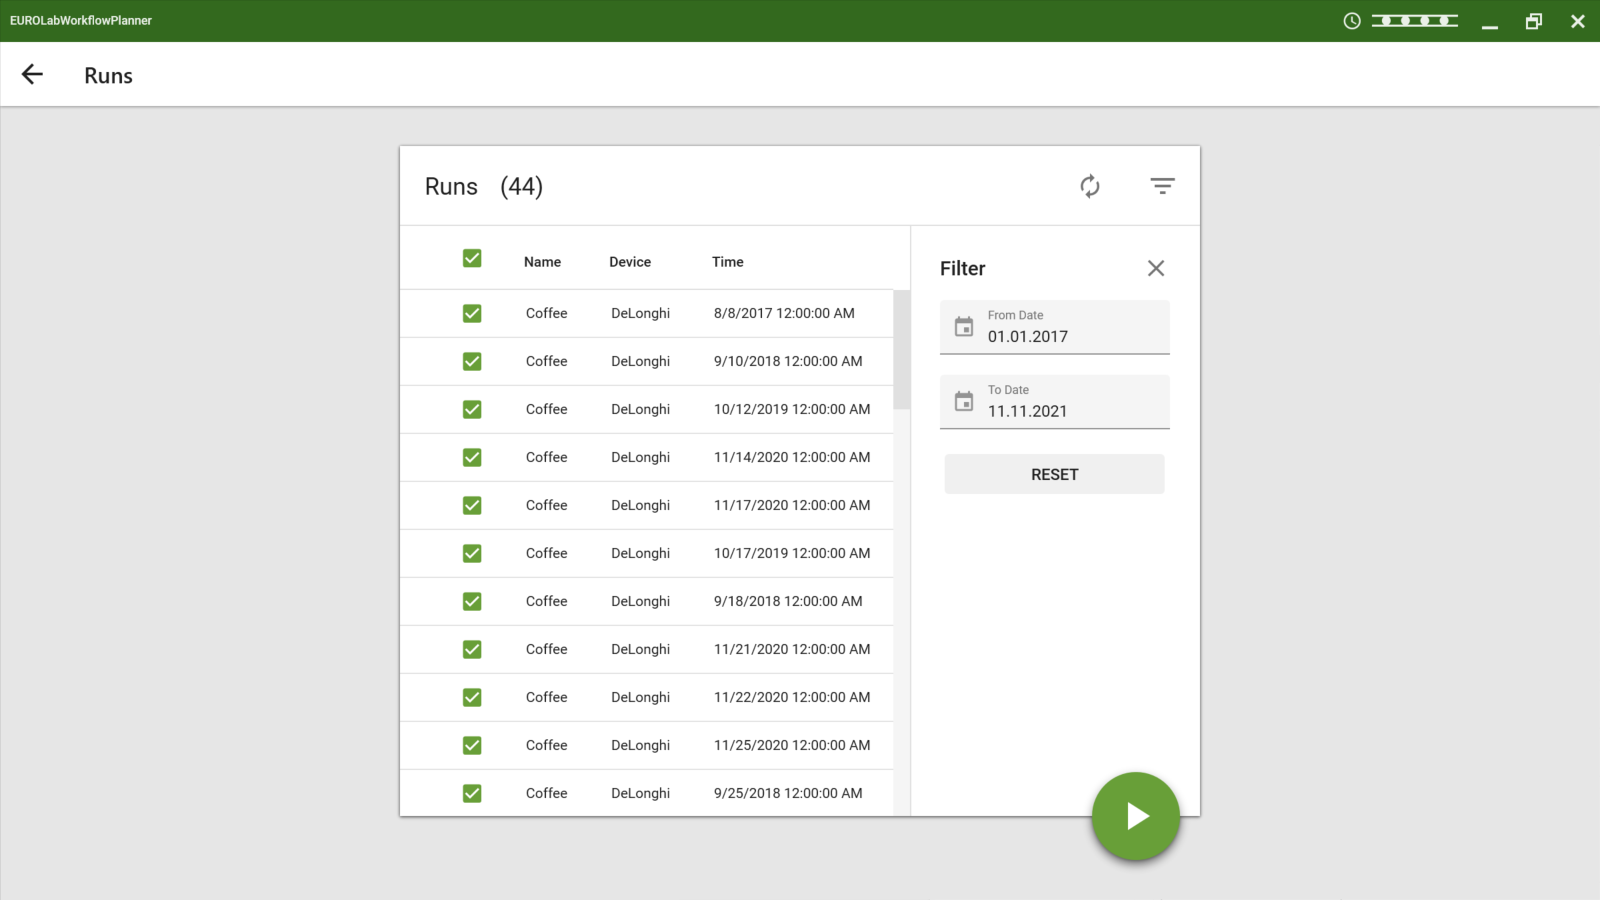
\includegraphics[scale=0.5]{Bilder/RunsAnsicht.png}
	\caption{Hauptansicht der abgefragten Daten}
	\label{fig:Runs}
\end{figure} 

\subsection{Implementierung der Geschäftslogik}
\label{sec:ImplementierungDerGeschäftslogik}
Die Implementierung der Schnittstelle via {\acs{gRPC}} wurde vom Betrieb vorgegeben, da die Technologie an anderen Stelle bereits verwendet wurde und somit ein gewisses Grundwissen vorhanden war.

Zunächst war das Ziel eine Schnittstelle zu entwickeln, die einfach von anderen Gerätesoftware-Projekten implementiert werden kann. Diese Schnittstelle wird entwickelt und in ein {\acs{NuGet}}-Paket ausgelagert. Durch die Nutzung eines firmeninternen {\acs{GitLab}}-Servers wird dieses Paket für die firmeninterne Nutzung freigegeben.

Zur Implementierung dieser Schnittstelle muss die Klasse \glqq RPCServer\grqq \space (s. Listing~\ref{app:ServerseitigeKlasse}) initialisiert werden. In den Konstruktor wird dazu das Interface \glqq IEUROLabWorkflowPlannerService\grqq \space (s. Listing~\ref{app:Schnittstelle}) rein gereicht. Über eine eigene Implementierung des Interfaces können die Daten entsprechend der Software des Diagnostikgeräts erbracht werden.

Bei Abfrage der Daten werden ein Anfangsdatum und ein Enddatum übergeben, sodass der Server nur Daten im entsprechenden Zeitrahmen zurück sendet. Außerdem werden Verbräuche mit Verbrauchsnamen gekennzeichnet. Anhand dieser Namen werden gleichnamige zusammengerechnet und zur besseren Übersicht gegliedert (s. Abbildung~\ref{fig:Consumptions}). Eine qualitative Bewertung der Daten findet nicht statt, die Daten werden unabhängig von Einheiten verarbeitet.

\begin{figure}[htb]
	\centering
	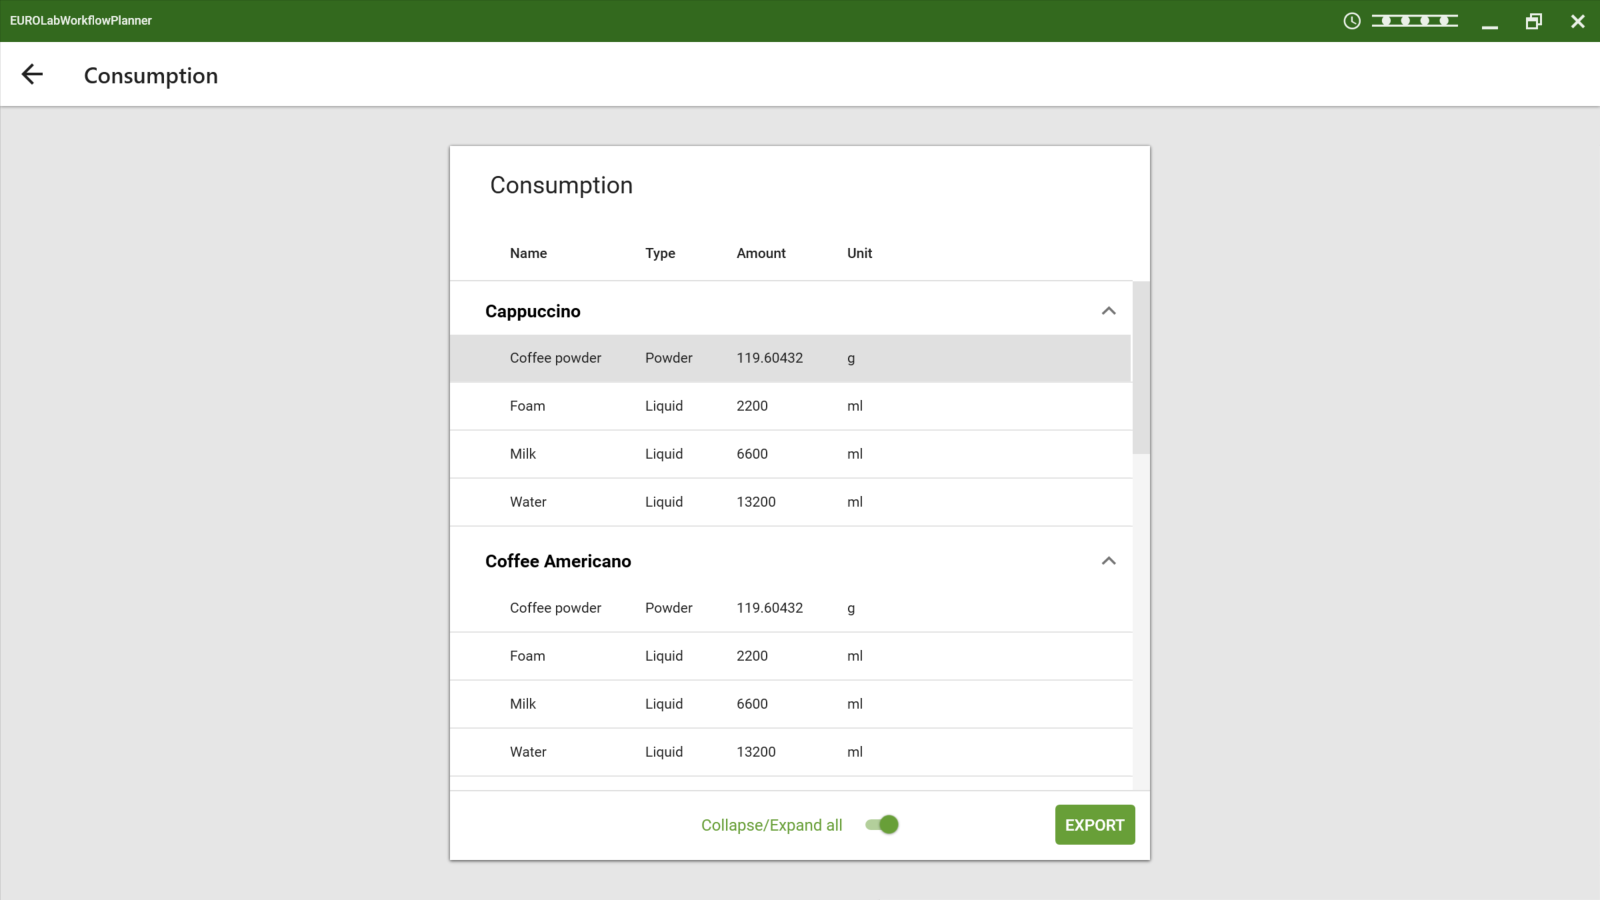
\includegraphics[scale=0.5]{Bilder/VerbrauchAnsicht.png}
	\caption{Ansicht der zusammengefassten Betriebsmittelverbräuche}
	\label{fig:Consumptions}
\end{figure}